\chapter{Dataset study}

\section{Generating data}
We generate the dataset by simulating various sheet cut configuratations under
multiple combinations of normal load and stretch. For each configuration we
sample 15 pseudo uniform (\hl{refer to relevant section here}) strech values
between zero and the rupture stretch found in the rupture test. The normal force
is uniformly sampled in the range $[0.1, 10]$ nN. In total this gives $3\times
15$ data points for each configuration. For the remaining parameters we use the
values presented in the pilot study (see table \ref{tab:param}). We generate 68
configurations of the Tetrahedron pattern type, 45 of the Honeycomb type and 100
of the Random walk type which is shown in \hl{Appendix C?}. A summary of the
data points is given in table \ref{tab:dataset_summary}. The table shows that
not all submitted data points ``makes it'' to the final dataset. This is due to
the combination of our numerical procedure and small variations in the rupture
stretch point. After performing the rupture test the simulation is restarted
with a new substrate size corresponding to the measured rupture stretch limit
and also with new random velocity and thermostat initializations values. The sheet is then stretched and checkpoints of the simulation state (LAMMPS restart files) are saved for each of the targeted stretch samples. However, if the rupture points arrives slightly early than syggested by the rupture test, some sampled stretch values might not get a corresponding checkpoint file. Thus, these data points are not included in the data set even though they ideally should have been noted as a rupture event. This could quite easily have been mittigated by a rewrite of that part of the code, but it was first discovered after the dataset had been created. However, the dataset still includeds 11.57 \% rupture events and it most likely that the most cases with a lost rupturer event have a rupture event stored for the preeceding stretch value instead which captures the information of the sheet stretch limit on its own. 

\begin{table}[H]
  \begin{center}
  \caption{Summary of the number of generated data points in the dataset. Due to slight deviations in the rupture stretch and the specific numerical procedure not all submitted simulations ``makes it'' to the final dataset. Notice that the Tetrahedon (7, 5, 2) and Honeycomb (2, 2, 1, 5) from the pilot study is rerun as a part of the Tetrahedon and the Honeycomb datasets seperately. In the latter datasets the reference point for the pattern is randomized and thus theese configurations is not fully identical. This is the idea behind the difference of 2 in the total sum.}
  \label{tab:dataset_summary}
  \begin{tabular}{ | c | c | c | c | c |} \hline
  \textbf{Type} & \textbf{Configurations} & \textbf{Submitted data points} & \textbf{Final data points} & \textbf{Ruptures} \\ \hline
  Pilot study & 3 & 270 & 261 & \: 25 \: (9.58 \%)\\ \hline
  Tetrahedon & 68 & 3060 & 3015 & 391 (12.97 \%)\\ \hline
  Honeycomb & 45 & 2025 & 1983 & \: 80 \: (4.03 \%)\\ \hline
  Random walk & 100 & 4500 & 4401 & 622 (14.13 \%) \\ \hline \hline
  Total & 214 (216) & 9855 & 9660 & 1118 (11.57 \%) \\ \hline
  \end{tabular}
  \end{center}
\end{table}


\section{Data analysis}


In order to gain insight into the correlations between variables associated to the simulations we calculate the correlations coefficients between all variable combinations. More specific, we are going to calculate the Pearson product-moment correlation coefficient (PPMCC) for which is defined, between data set $X$ and $Y$, as
\begin{align*}
  \mathrm{corr}(X,Y) = \frac{\mathrm{Cov}(X,Y)}{\sigma_X \sigma_Y} = \frac{\langle (X - \mu_X)(Y - \mu_Y)\rangle}{\sigma_X \sigma_Y} \ \in [-1, 1]
\end{align*}
where $\mathrm{Cov}(X,Y)$ is the covariance, $\mu$ the mean value and $\sigma$ the standard deviation. The correlation coefficients ranges from perfect negative correlation $(-1)$ through no correlation $(0)$ to a perfect positive correlation $(1)$. The correlation coefficients is shown in figure \ref{fig:corrcoef_matrix}

\begin{figure}[H]
  \centering
  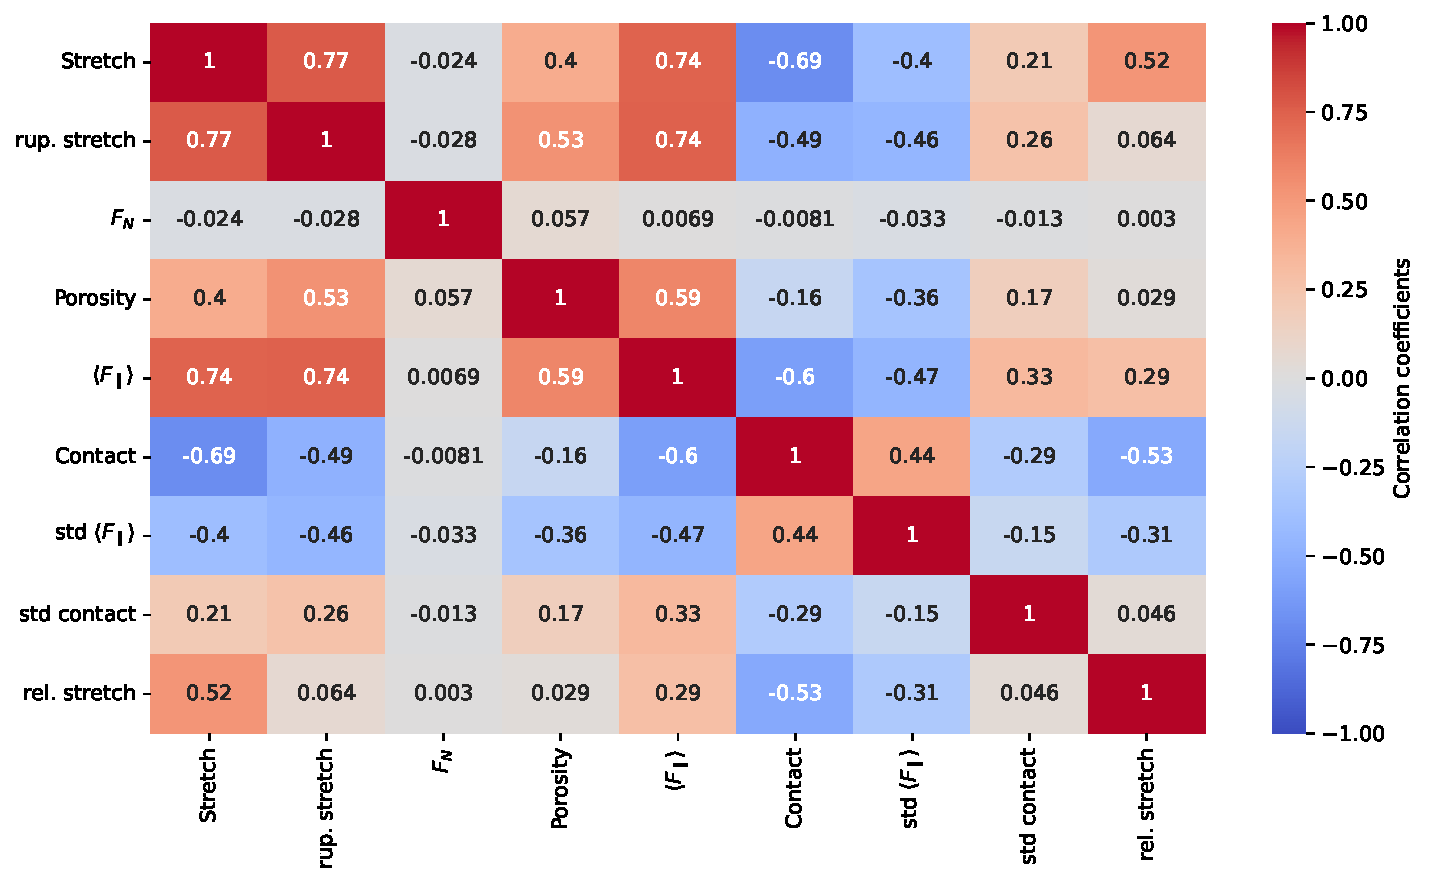
\includegraphics[width=\linewidth]{figures/ML/corrcoef_matrix.pdf}
  \caption{Pearson product-moment correlation coefficients for the full datset (see table \ref{tab:dataset_summary}).}
  \label{fig:corrcoef_matrix}
\end{figure}

From figure \ref{fig:corrcoef_matrix} we especially notice that the mean
friction force $\langle F_{\parallel} \rangle$ has a signifciant positively
correlation with stretch $(0.77)$ and porosity $(0.60)$ (void fraction).
However, the relative stretch, which is scaled by the rupture stretch, has a
weaker correlation of only 0.25 which indicates that it is the absolute stretch
value that has the most significant impact on the friction force increase during
stretching. This is further supported by the fact that the mean friction and the
rupture stretch is also strongly positively correlated $(0.78)$. From figure
\ref{fig:corrcoef_matrix} we also observe that the contact bond count is
negatively correlated with the mean friction $(-0.67)$ and the stretch value
$(-0.74)$ which is consistent with the trend observed in the pilot study (figure \ref{fig:multi_stretch_contact} and \ref{fig:multi_stretch_mean_fric}) of the
contact decreasing with increasing stretch and mean friction. However, we must
take note that the correlation coefficients is a measure of the strength and slope of a
forced linear fit on the data. We clearly observed a non-linear relationship between stretch and mean friction for the tetrahedron and honeycomb pattern used in the pilot study (figure \ref{fig:multi_stretch_mean_fric}) where the relationship was partwise characterized by a postive correlation for some stretch ranges and partwise negative correlation for other stretch ranges. Hence, interesting strong regime-specific correlations might not be accurately highlighted by the correlation coefficients shown in figure \ref{fig:corrcoef_matrix}.

In figure \ref{fig:corr_vis} we have visualized the data (excluding the pilot study) for chosen pairs of variables on the axes. In addition to a visual confirmation of how the given correlations look in a 2D plot we also get a feeling for the coverage in various areas of the parameter space that we are eventually going to feed the neural network. The honeycomb pattern is spanning a significant larger range of stretch, contact and mean friction makes the data rather biased towards the Honeycomb pattern in thoose areas. 
% Judging form the combinned information of the pilot study and the data distribution shown in figure \ref{fig:corr_vis} it would not be surprising if the machine learning were to learn that the honeycomb pattern is superiour for 

\begin{figure}[H]
  \centering
  \begin{subfigure}[t]{0.49\textwidth}
      \centering
      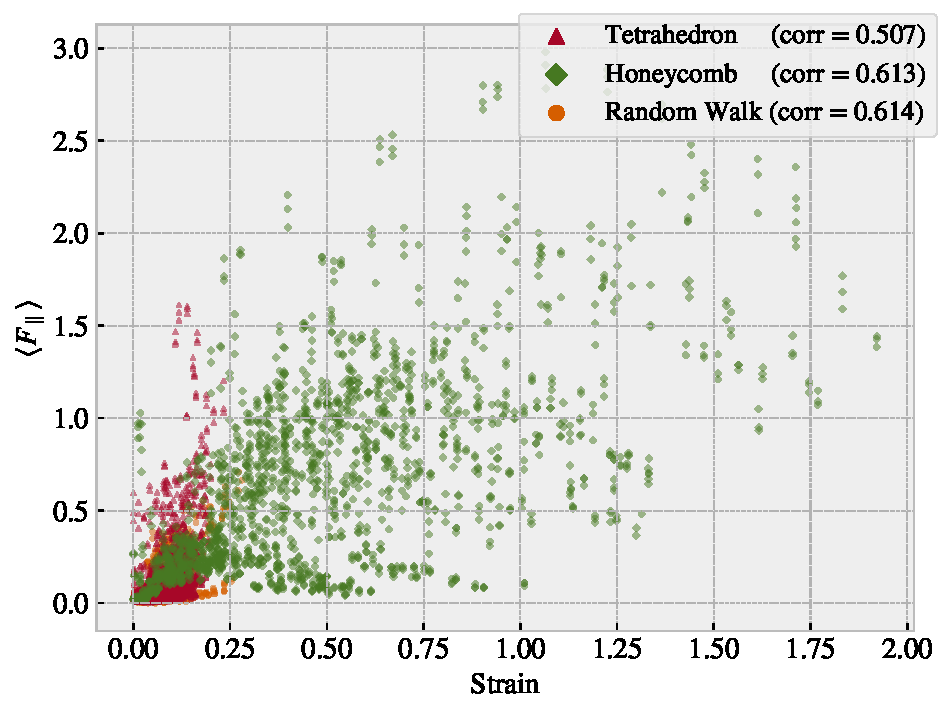
\includegraphics[width=\textwidth]{figures/ML/corr_stretch_Ff.pdf}
      \caption{}
      % \label{fig:}
  \end{subfigure}
  \hfill
  \begin{subfigure}[t]{0.49\textwidth}
      \centering
      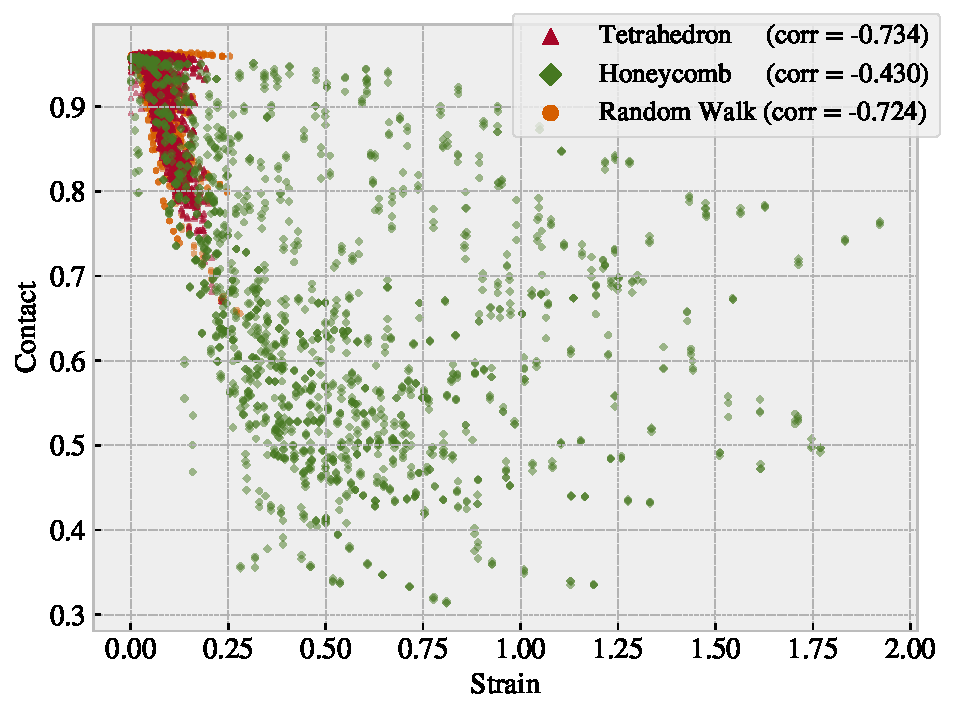
\includegraphics[width=\textwidth]{figures/ML/corr_stretch_contact.pdf}
      \caption{}
      % \label{fig:}
  \end{subfigure}
  \hfill
  \begin{subfigure}[t]{0.49\textwidth}
      \centering
      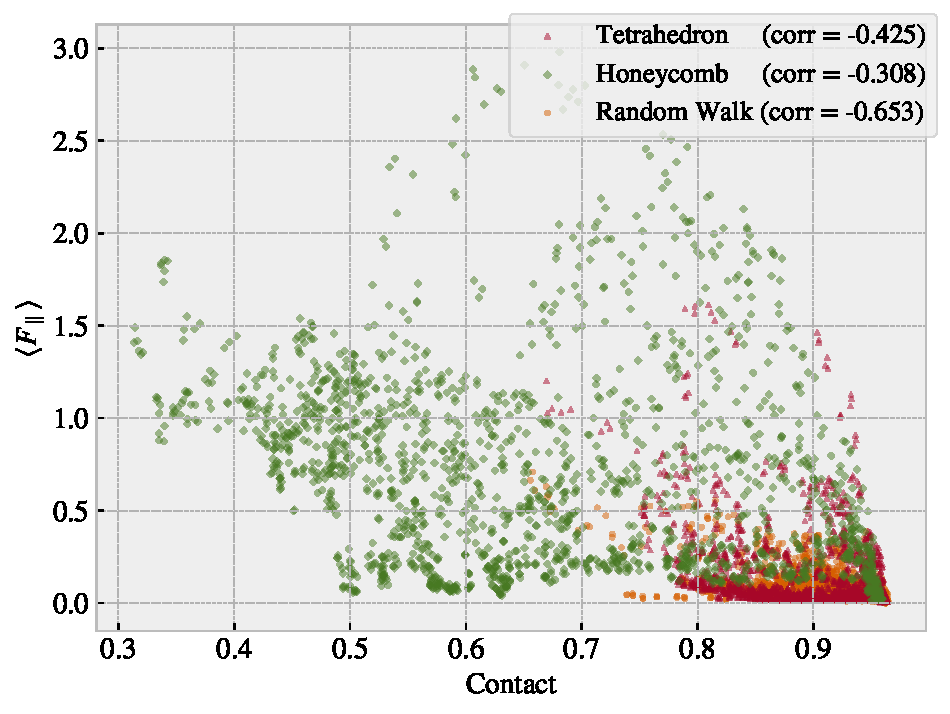
\includegraphics[width=\textwidth]{figures/ML/corr_contact_Ff.pdf}
      \caption{}
      % \label{fig:}
  \end{subfigure}
  \hfill
  \begin{subfigure}[t]{0.49\textwidth}
      \centering
      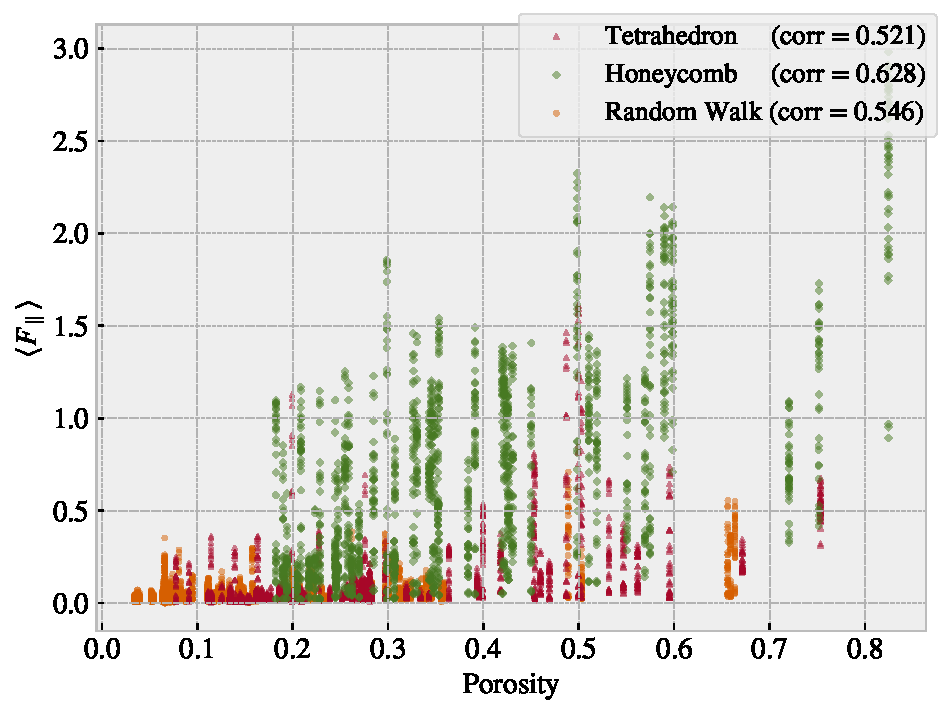
\includegraphics[width=\textwidth]{figures/ML/corr_porosity_Ff.pdf}
      \caption{}
      % \label{fig:}
  \end{subfigure}
  \hfill
     \caption{Scatter plot of the data sets Tetrahedron, Honeycomb and Random Walk (excluding the pilot study) for various variable combinations in order to visualize some chosen  correlations of interest and distributions in the data}
     \label{fig:corr_vis}
\end{figure}


\section{Properties of interest / Stretch profiles}
\hl{Define somewhere that we will look at low friction, high friction and the biggest (forward) drop in friction corresponding to a significant negative friction coefficient}.



\begin{table}[H]
  \begin{center}
  \caption{Interesting properties}
  \label{tab:}
  \begin{tabular}{| c | c | c | c|} \hline
  \textbf{Tetrahedron} & Configuration & Stretch & Value [nN]  \\ \hline
  Min $F_{\text{fric}}$ & $(3,9,4)$ &  0.0296 & 0.0067 \\ \hline
  Max & $(5,3,1)$ & 0.1391 & 1.5875 \\ \hline
  Max $\Delta F_{\text{fric}}$  & $(5, 3, 1)$ & $[0.0239, 0.1391]$ & 1.5529 \\ \hline
  Max drop & $(5,3,1)$ & $[0.1391, 0.1999]$ & 0.8841 \\ \hline
  \multicolumn{4}{c}{} \\ \hline
  % \textbf{Tetrahedron} & \multicolumn{3}{c|}{} \\ \hline
  \textbf{Honeycomb} & Configuration & Stretch & Value [nN]  \\ \hline
  Min $F_{\text{fric}}$ & $(2, 5, 1, 1)$ &  0.0267 & 0.0177 \\ \hline
  Max & $(2, 1, 1, 1)$ & 1.0654 & 2.8903 \\ \hline
  Max $\Delta F_{\text{fric}}$  & $(2, 1, 5, 3)$ & $[0.0856, 1.4760]$ & 2.0234 \\ \hline
  Max drop & $(2, 3, 3, 3)$ & $[0.5410, 1.0100]$ & 1.2785 \\ \hline
  \multicolumn{4}{c}{} \\ \hline
  \textbf{Random walk} & Configuration & Stretch & Value [nN]  \\ \hline
  Min $F_{\text{fric}}$ & 12 &  0.0562 & 0.0024\\ \hline
  Max & 96 & 0.2375 & 0.5758 \\ \hline
  Max $\Delta F_{\text{fric}}$  & 96 & $[0.0364, 0.2375]$ & 0.5448 \\ \hline
  Max drop & 01 & $[0.0592, 0.1127]$ & 0.1818 \\ \hline
\end{tabular}
\end{center}
\end{table}


% Popup
% ['(3, 9, 4)', 0.0296407442523106, 0.006738434728040425]
% ['(5, 3, 1)', 0.139120019152679, 1.5874991413277917]
% ['(5, 3, 1)', 0.0238700191526787, 0.139120019152679, 1.5529155085058322]
% ['(5, 3, 1)', 0.139120019152679, 0.199920019152683, 0.8840614643066859]

% Honeycomb
% ['(2, 5, 1, 1)', 0.0267215709876031, 0.01771035812444661]
% ['(2, 1, 1, 1)', 1.06536290170726, 2.8903313732271183]
% ['(2, 1, 5, 3)', 0.085589883539189, 1.47601988353919, 2.023377918411005]
% ['(2, 3, 3, 3)', 0.541004661720013, 1.01001466172002, 1.278541503443495]

% RW
% ['12', 0.0562087686350666, 0.002350782025058632]
% ['96', 0.237523191134115, 0.5757864994802119]
% ['96', 0.0363631911341175, 0.237523191134115, 0.5447910475168634]
% ['01', 0.0591598822685843, 0.112739882268582, 0.18175926264779968]


\begin{figure}[H]
  \centering
  \begin{subfigure}[t]{0.49\textwidth}
      \centering
      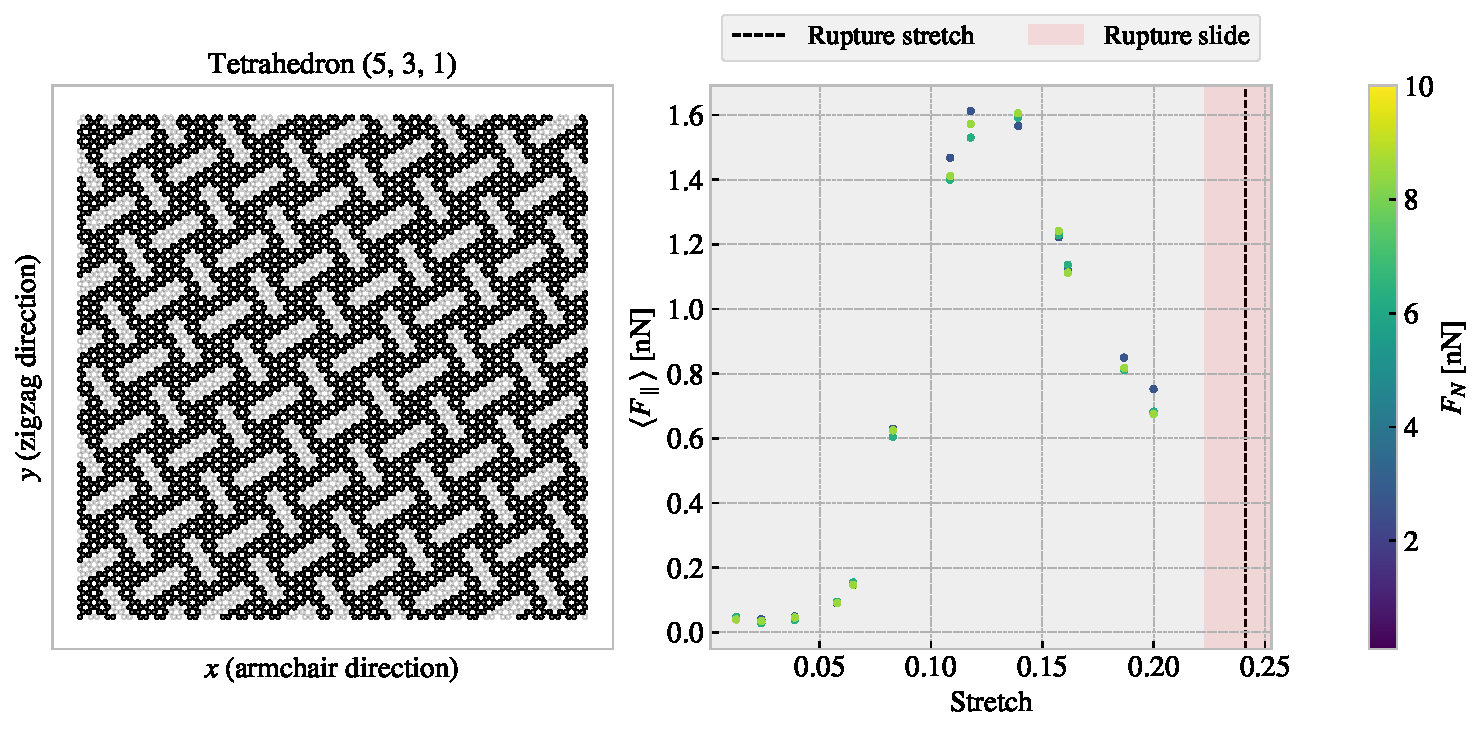
\includegraphics[width=\textwidth]{figures/stretch_profiles/PP_pop_27.pdf}
      \caption{}
  \end{subfigure}
  \hfill
  \begin{subfigure}[t]{0.49\textwidth}
      \centering
      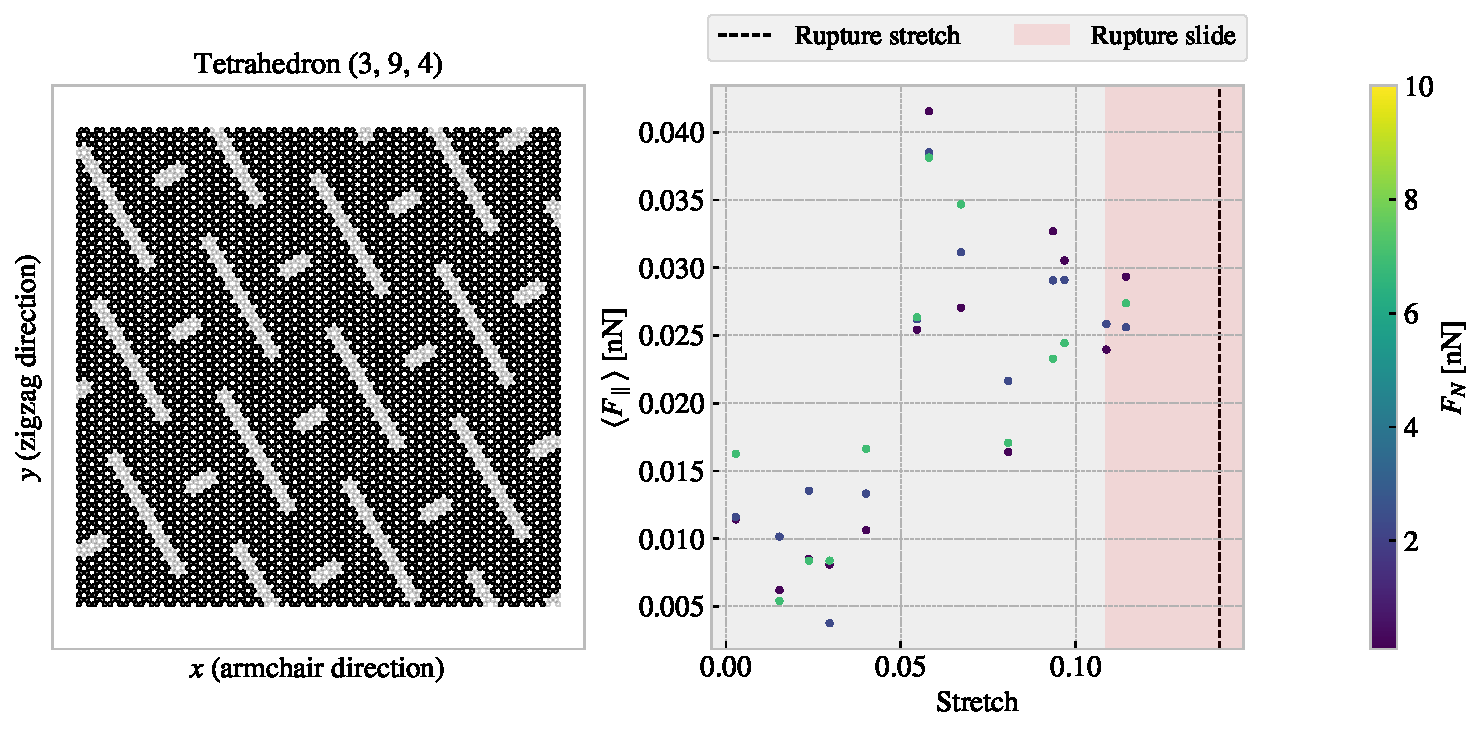
\includegraphics[width=\textwidth]{figures/stretch_profiles/PP_pop_31.pdf}
      \caption{}
  \end{subfigure}
  \hfill
  \begin{subfigure}[t]{0.49\textwidth}
      \centering
      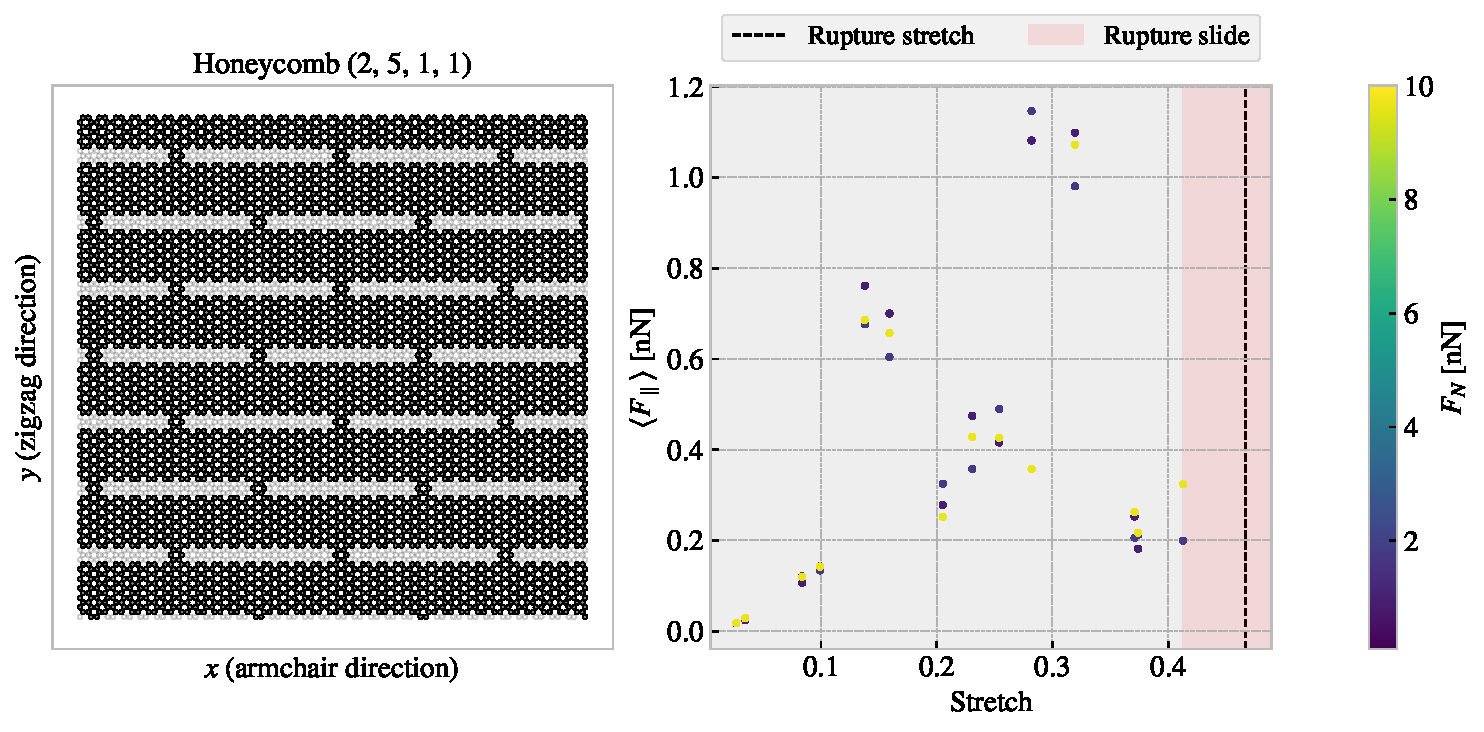
\includegraphics[width=\textwidth]{figures/stretch_profiles/PP_hon_6.pdf}
      \caption{}
  \end{subfigure}
  \hfill
  \begin{subfigure}[t]{0.49\textwidth}
      \centering
      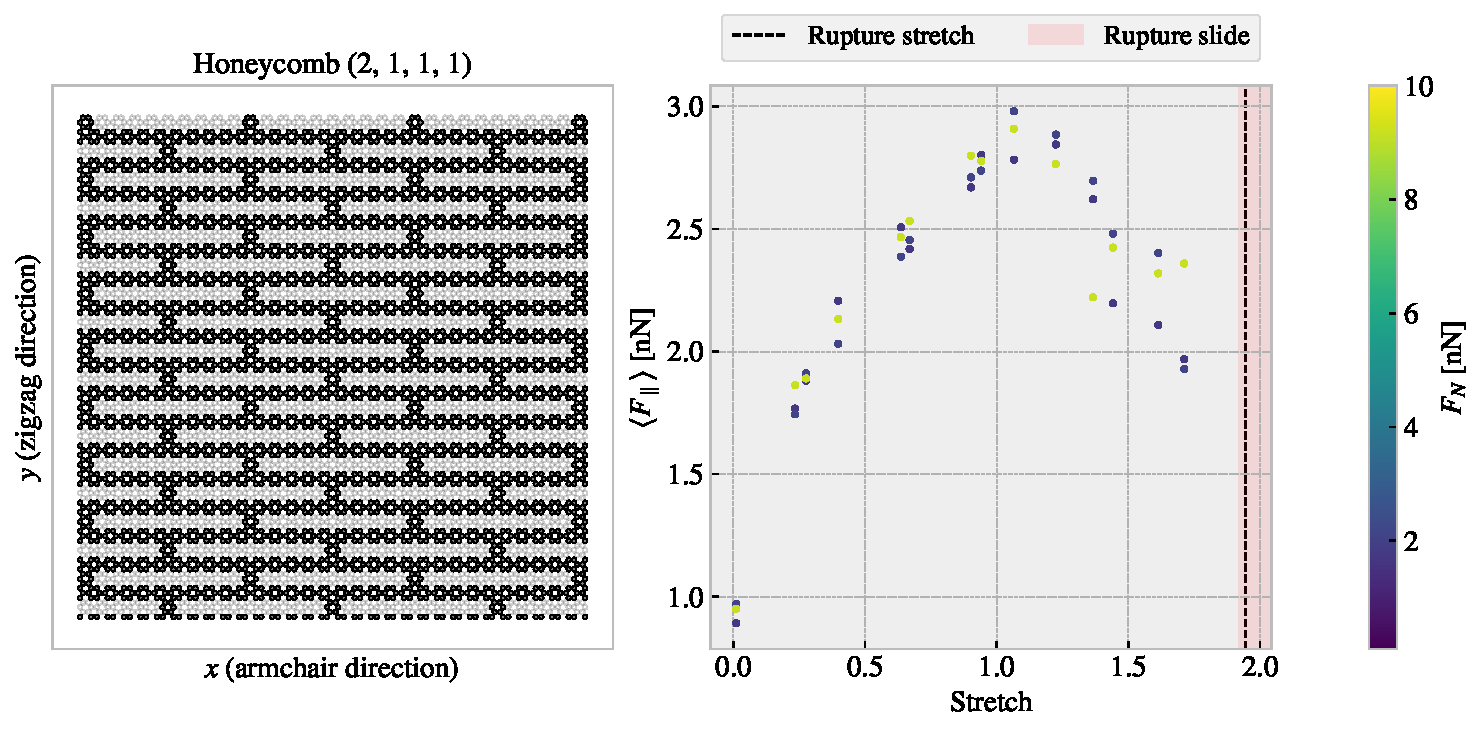
\includegraphics[width=\textwidth]{figures/stretch_profiles/PP_hon_12.pdf}
      \caption{}
  \end{subfigure}
  \hfill
  \begin{subfigure}[t]{0.49\textwidth}
      \centering
      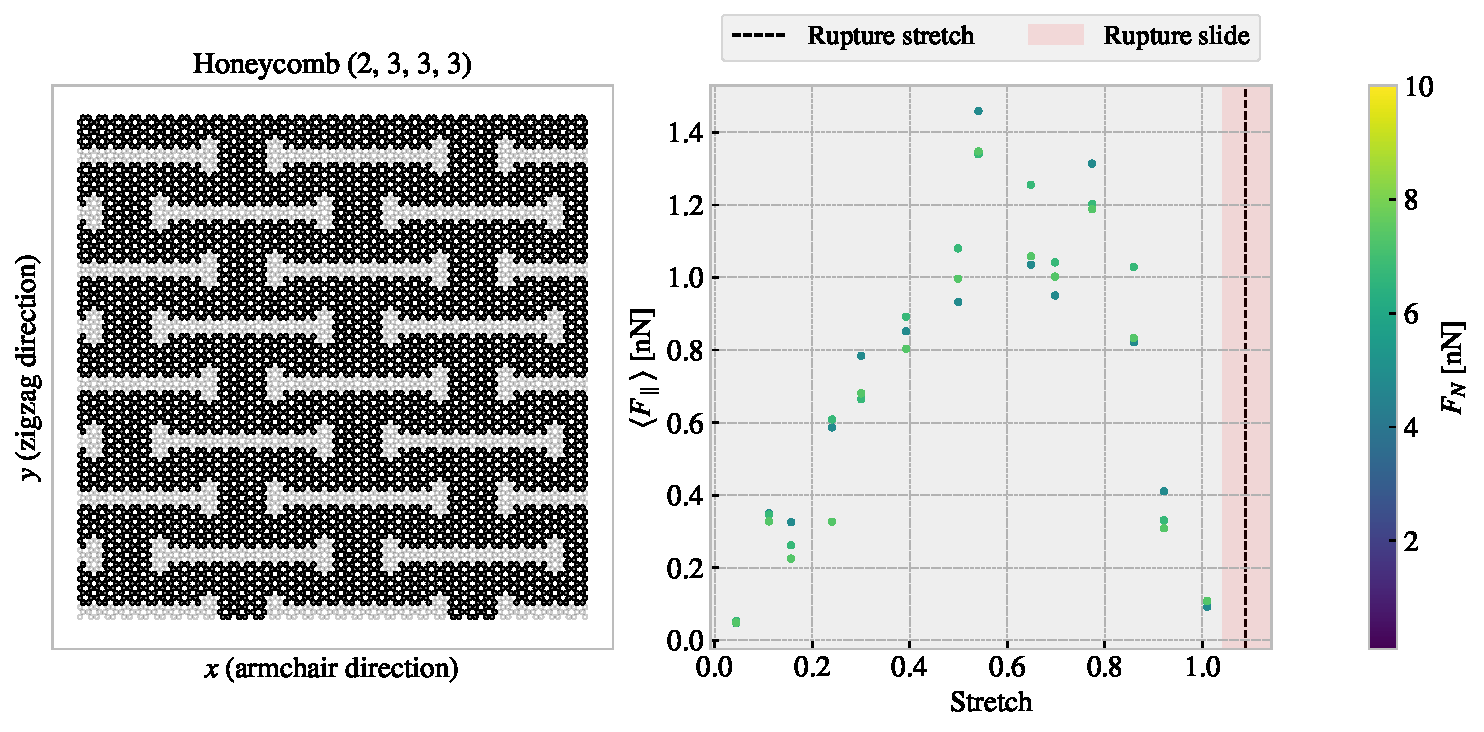
\includegraphics[width=\textwidth]{figures/stretch_profiles/PP_hon_28}
      \caption{}
  \end{subfigure}
  \hfill
  \begin{subfigure}[t]{0.49\textwidth}
      \centering
      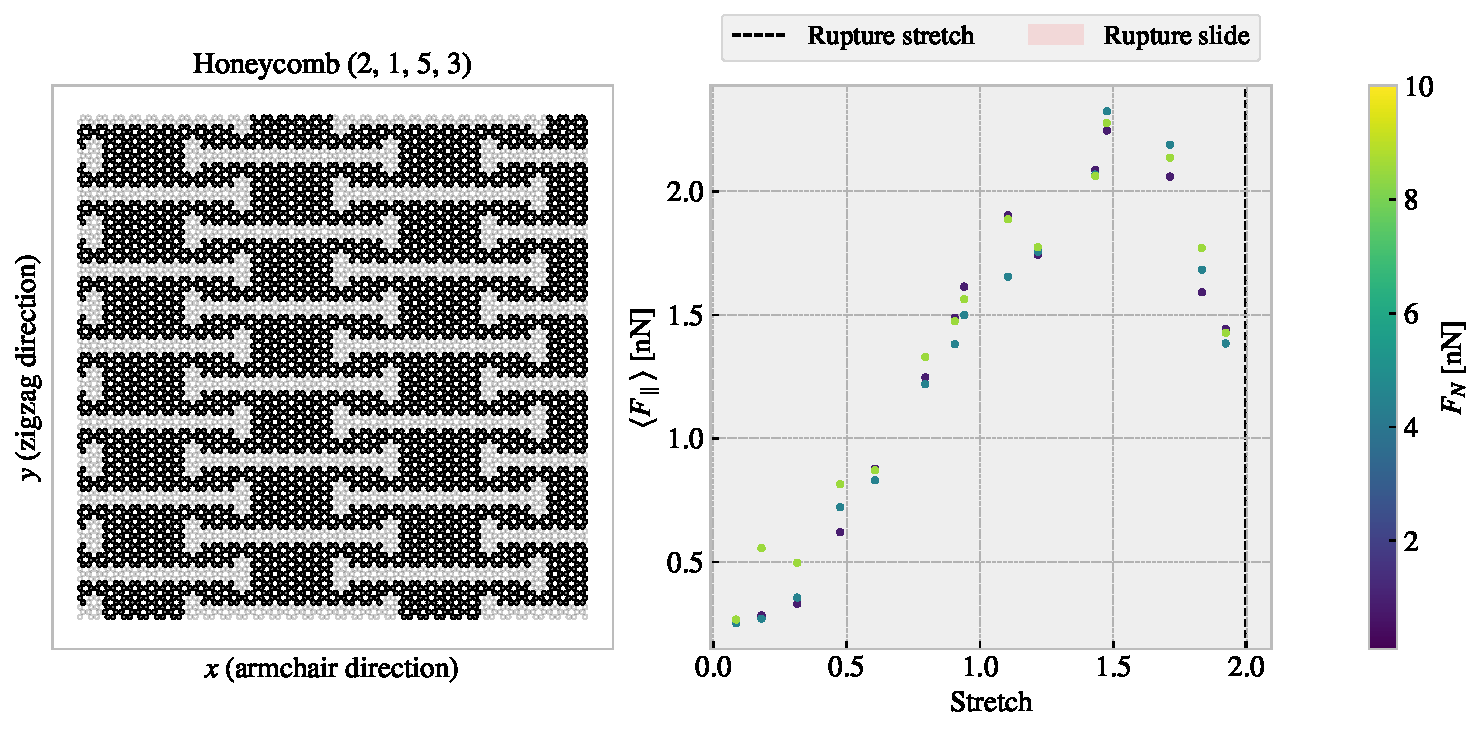
\includegraphics[width=\textwidth]{figures/stretch_profiles/PP_hon_42.pdf}
      \caption{}
  \end{subfigure}
  \hfill
  \begin{subfigure}[t]{0.49\textwidth}
      \centering
      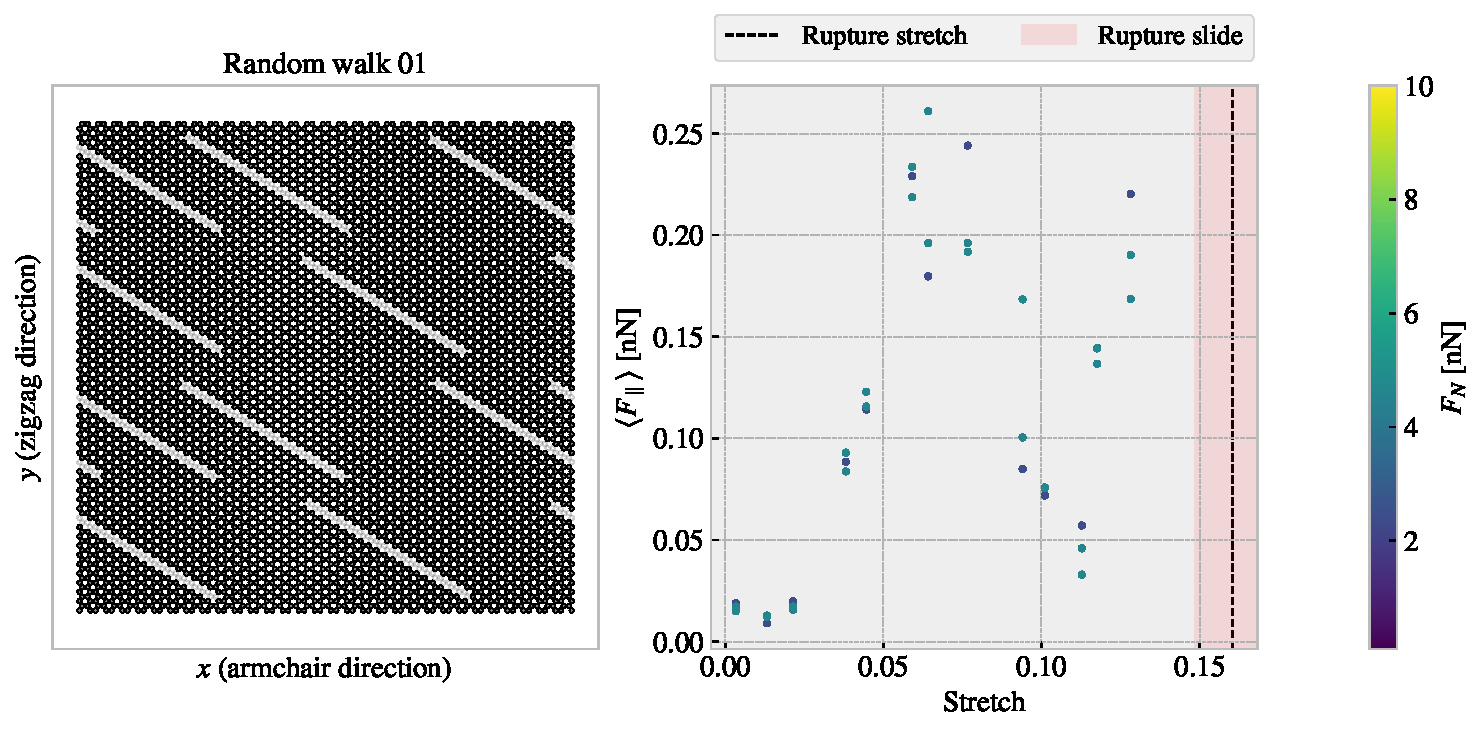
\includegraphics[width=\textwidth]{figures/stretch_profiles/PP_RW01.pdf}
      \caption{}
  \end{subfigure}
  \hfill
  \begin{subfigure}[t]{0.49\textwidth}
      \centering
      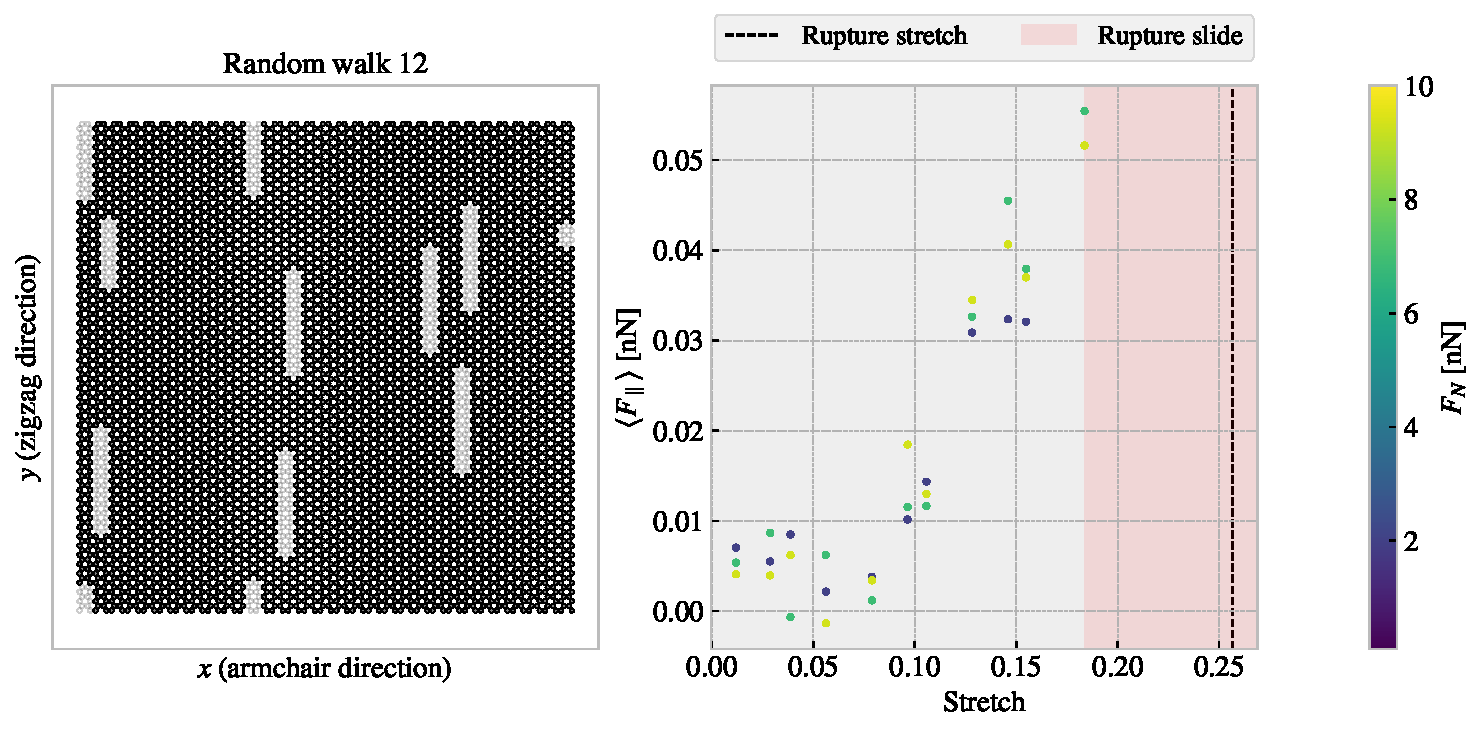
\includegraphics[width=\textwidth]{figures/stretch_profiles/PP_RW12.pdf}
      \caption{}
  \end{subfigure}
  \hfill
  \begin{subfigure}[t]{0.49\textwidth}
      \centering
      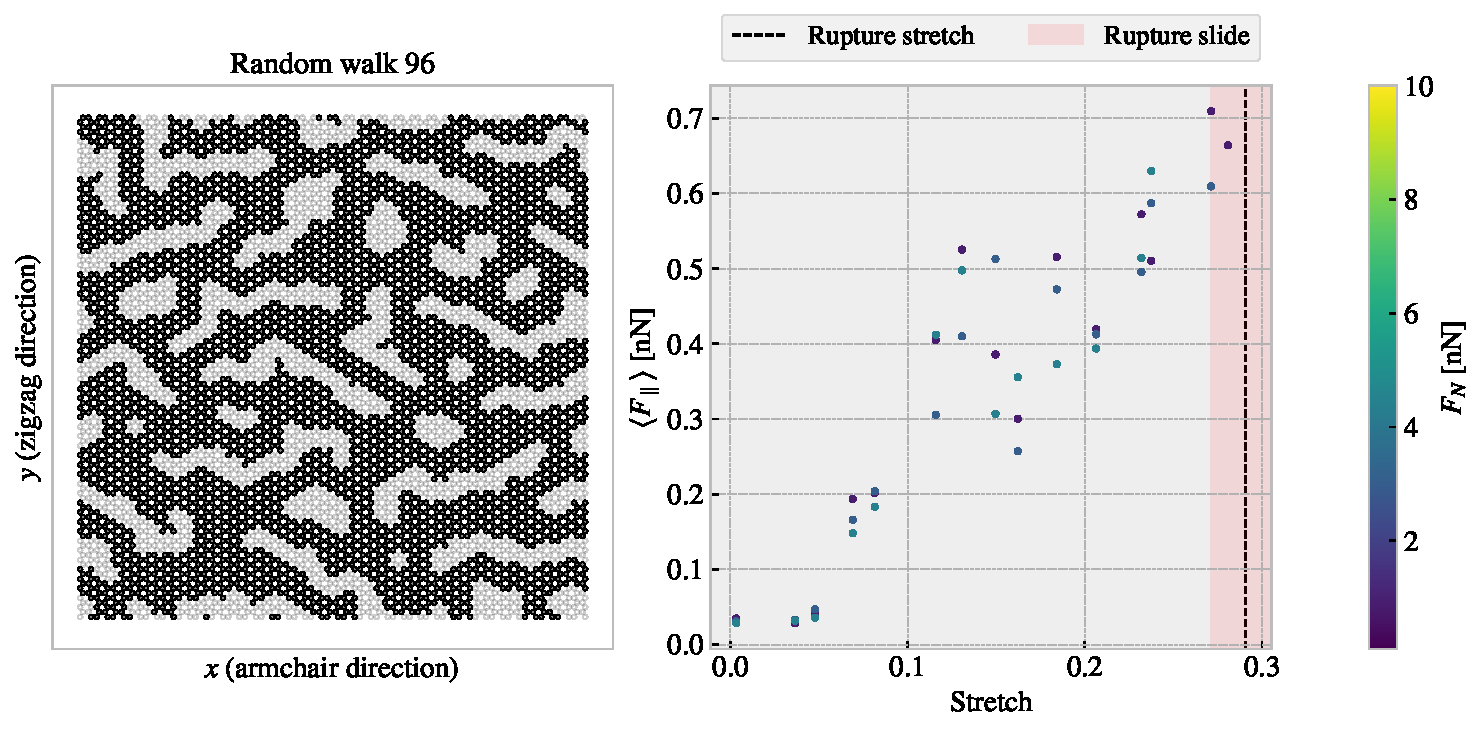
\includegraphics[width=\textwidth]{figures/stretch_profiles/PP_RW96.pdf}
      \caption{}
  \end{subfigure}
  \hfill
     \caption{}
     \label{fig:}
\end{figure}






The stretch profiles for all the configurations are shown in appendix \ref{sec:data_stretch_profiles}.


\section{Machine learning}

Staircase architecture tuning.



 
\section{Accelerated Search}

Having a network model that can predict friction force for a given configuration are able to search for some desired properties. Low and high friction and maximal negative friction coefficeints


Here we pursue two different approaches for finding 
\begin{enumerate}
  \item Generate an enlarged dataset and run it through the ML model 
  \item Genetic algorithm
\end{enumerate}


\subsection{Markov-Chain Accelerated Genetic Algorithms}
% Following the article:
% Accelerated Genetic Algorithms with Markov Chains
% Guan Wang, Chen Chen, and K.Y. Szeto

\subsubsection{Talk about traditional method also?}

\subsubsection{Implementing for 1D chromosone (following article closely)}

We have the binary population matrix $A(t)$ at time (generation) $t$ consisting of $N$ rows denoting chromosones and with $L$ columns denoting the so-called locus (fixed position on a chromosome where a particular gene or genetic marker is located, wiki). We sort the matrix rowwise by the fitness of each chromosono evaluated by a fitness function $f$ such that $f_i(t) \le f_k(t)$ for $i \ge k$. We assume that there are a transistion probability between the current state $A(t)$ and the next state $A(t+1)$. We consider this transistion probability only to take into account mutation process (mutation only updating scheme). During each generation chromosones are sorted from most to least fitted. The chromosone at the $i$-th fitted place is assigned a row mutation probability $a_i(t)$ by some monotonic increasing function. This is taken to be 
\begin{align*}
  a_i(t) = 
  \begin{cases}
    (i-1)/N',& i-1 < N' \\
    1, &\text{else}
  \end{cases}
\end{align*}
for some limit $N'$ (refer to first part of article talking about this). We use $N' = N/2$. We also defines the survival probability $s_i = 1 - a_i$. In thus wau $a_i$ and $s_i$ decide together whether to mutate to the other state (flip binary) or to remain in the current state. We use $s_i$ as the statistical weight for the $i$-th chromosone given it a weight $w_i = s_i$.
\\
Now the column mutation. For each locus $j$ we define the count of 0's and 1's as $C_0(j)$ and $C_1(j)$ resepctively. These are normalized as
\begin{align*}
  n_0(j, t) = \frac{C_0(j)}{C_0(j) + C_1(j)}, \quad n_1(j, t) = \frac{C_1(j)}{C_0(j) + C_1(j)}.
\end{align*}
These are gathered into the vector $\vec{n}(j,t)=(n_0(j, t), n_1(j, t))$ which characterizes the state distribution of $j$-th locus. In order to direct the current population to a preferred state for locus $j$ we look at the highest weight of row $i$ for locus $j$ taking the value 0 and 1 respectively.
\begin{align*}
  C'_0(j) &= \max\{W_i | A_{ij} = 0; \ i = 1, \cdots, N\} \\
  C'_1(j) &= \max\{W_i | A_{ij} = 1; \ i = 1, \cdots, N\}
\end{align*}
which is normalized again
\begin{align*}
  n_0(j, t+1) = \frac{C'_0(j)}{C'_0(j) + C'_1(j)}, \quad n_1(j, t+1) = \frac{C'_1(j)}{C'_0(j) + C'_1(j)}.
\end{align*}
The vector $\vec{n}(j,t+1)=(n_0(j, t+1), n_1(j, t+1))$ then provides a direction for the population to evolve against. This characterizes the target state distribution of the locus $j$ among all the chromosones in the next generation. We have
\begin{align*}
  \begin{bmatrix}
    n_0(j, t+1) \\
    n_1(j, t+1)
  \end{bmatrix}
  = 
  \begin{bmatrix}
    P_{00}(j,t) \ P_{10}(j,t) \\
    P_{01}(j,t) \ P_{11}(j,t)
  \end{bmatrix}
  \begin{bmatrix}
    n_0(j, t) \\
    n_1(j, t)
  \end{bmatrix}
\end{align*}
Since the probability must sum to one for the rows in the P-matrix we have 
\begin{align*}
  P_{00}(j, t) = 1 - P_{01}(j, t), \quad P_{11}(j, t) = 1 - P_{10}(j, t)
\end{align*}
These conditions allow us to solve for the transition probability $P_{10}(j,t)$ in terms of the single variable $P_{00}{j,t}$.
\begin{align*}
  P_{10}(j,t) &= \frac{n_0(j, t+1) - P_{00}(j,t)n_0(j, t)}{n_1(j,t)} \\
  P_{01}(j,t) &= 1 - P_{00}(j,t) \\
  P_{11}(j,t) &= 1 - P_{10}(j,t)
\end{align*}
We just need to know $P_{00}(j,t)$. We start from $P_{00}(j, t = 0) = 0.5$ and then choose $P_{00}(j,t) = n_0(j,t)$




